\icode{N23S-MCC-CA-L2-261025-001}
\nceeID[6]{2023江苏}{13}
“转碟”是传统的杂技项目。如图所示，质量为\(m\)的发光物体放在半径为\(r\)的碟子边缘，杂技演员用杆顶住碟子中心，使发光物体随碟子一起在水平面内绕\(A\)点做匀速圆周运动。当角速度为\(\omega_0\)时，碟子边缘看似一个光环。求此时发光物体的速度大小\(v_0\)和受到的静摩擦力大小\(f\)。

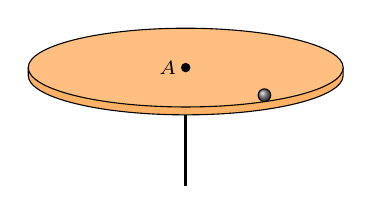
\begin{tikzpicture}[font=\scriptsize]
	\draw[very thick] (0,0)--(0,-1.5);
    \draw[fill=orange!60] (-2,0)--(-2,-.1) arc(180:360: 2 and .5)--(2,0);
    \draw[fill=orange!50] (0,0) ellipse(2 and .5);
	\fill (0,0)node[left]{\(A\)} circle(.06);
	\draw[ball color=gray] (1,-.35) circle(.08);
\end{tikzpicture}
\begin{answer}
	\(v_0 = \omega_0r\)、\(f = m\omega_0^2r\)
\end{answer}